\hkapitola{Datové proudy}

\begin{frame}[fragile]
\frametitle{string}

\begin{block}{<string>}
\begin{itemize}
\item třída string je realizována šablonou \lstinline|basic_string<char>|
\item rozhraní zapadá do konceptu STL kontejnerů (viz později), chová se jako kontejner znaků
\item umožňuje jednodušše upravovat, vyhledávat, procházet řetězec
\end{itemize}
\end{block}

\begin{yesblock}
\begin{lstlisting}
string s1 = "hello world";
string s2{ "hello world" };
string s3 = s2;
string s4 = s1 + s2;

cout << s4.c_str() << endl;
\end{lstlisting}
\end{yesblock}
\end{frame}


\begin{frame}[fragile]
\frametitle{string -- základní metody a vlastnosti}

\begin{block}{}
\begin{itemize}
\item \lstinline|operator[]| -- procházení znaků
\item \lstinline|c_str()| -- konverze na \lstinline|const char*|
\item \lstinline|begin(), end()| -- iterátory
\item \lstinline|empty(), size()| -- test prázdnosti/test délky řetězce
\item \lstinline|insert(), erase()| -- vkládání, mazání znaků
\item \lstinline|substr()| -- výběr podřetězce
\item \lstinline|find(), rfind()| -- hledání podřetězce
\item \lstinline|find_first_of(), find_first_not_of()| -- hledání znaků
\item \lstinline|find_last_of(), find_last_not_of()| -- hledání znaků
\item porovávací operátory, \lstinline|replace()|, \lstinline|at()|, \lstinline|data()|, \ldots
\end{itemize}
\end{block}
\end{frame}


\begin{frame}[fragile]
\frametitle{Datové proudy}

\begin{block}{}
\begin{itemize}
\item nízkoúrovňové datové proudy zabaleny do objektů s jednoduchým rozhraním
\item proudy pro práci s konzolí, soubory a paměťový proud
\item jedná se o součást STL, ale neposkytují iterátorové rozhraní
\begin{itemize}
\item v knihovně jsou k dispozici adaptéry pro napojení na iterátory
\end{itemize}
\item vstup a výstup dat pomocí metod a přetížených operátorů (\lstinline|<<, >>|)
\end{itemize}
\end{block}


\begin{block}{}
\centering
\begin{tabular}{cccc}
\bfseries objekt & \bfseries instance třídy & \bfseries popis & \bfseries lowlevel proud (C) \\
\lstinline|cout| & \lstinline|ostream| & výstupní proud  & \lstinline|stdout| \\
\lstinline|cin| & \lstinline|istream| & vstupní proud & \lstinline|stdin| \\
\lstinline|cerr| & \lstinline|ostream| & chybový výstup & \lstinline|stderr| \\
\end{tabular}
\end{block}
\end{frame}





\begin{frame}[fragile]
\begin{yesblock}
\begin{lstlisting}
#include <iostream>
using namespace std;

int main(void)
{ 
	int cislo; 

	// výpis textu na obrazovku s odřádkováním
	cout << "Napis cislo" << endl; 
	// načtení celého čísla z klávesnice
	cin >> cislo; 

	cout << "Napsal jsi: " << cislo << endl; 
	return 0; 
}
\end{lstlisting}
\end{yesblock}
\end{frame}




\begin{frame}[fragile]
\frametitle{Manipulátory}
\begin{block}{}
\begin{itemize}
\item formát výstupu lze jednoduše přizpůsobit pomocí manipulátorů
\begin{itemize}
\item jednoduché objekty, které přenastaví proud
\end{itemize}
\item knihovna obsahuje řadu připravených manipulátorů
\begin{itemize}
\item lze definovat vlastní manipulátory
\end{itemize}
\item hlavičkový soubor \lstinline|<iomanip>|
\end{itemize}
\end{block}

\begin{yesblock}
\begin{lstlisting}
int val = 15;
cout << val << " 0x" << hex << val << endl;
// vypíše: 15 0xf
\end{lstlisting}
\end{yesblock}
\end{frame}






\begin{frame}[fragile]
\frametitle{Knihovní manipulátory}

\begin{block}{}
\begin{itemize}
\item \lstinline|endl| -- konec řádku a vyprázdnění bufferu
\item \lstinline|flush| -- vyprázdnění bufferu
\item \lstinline|dec, hex, oct| -- výpis čísel v desítkové, šestnáctkové nebo osmičkové soustavě
\item \lstinline|setbase(int)| -- výpis čísel v zadané soustavě
\item \lstinline|setw(int)| -- nastaví šířku vypisované hodnoty (na kolik znaků zarovnávat)
\item \lstinline|setfill(char)| -- nastaví vyplňovací znak
\item \lstinline|setprecision(int)| -- nastaví vypisovanou přesnost reálných čísel
\end{itemize}
\end{block}

\begin{yesblock}
\begin{lstlisting}[basicstyle=\small]
int c = 7;
cout << setw(3) << c << endl;
cout << setw(4) << setfill('@') << hex << c << endl;
\end{lstlisting}
\end{yesblock}
\end{frame}








\begin{frame}[fragile]
\frametitle{Hierarchie tříd proudů}

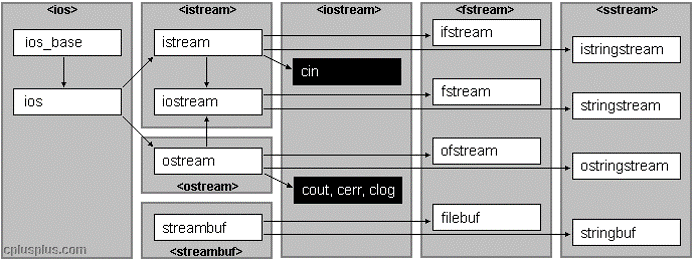
\includegraphics[width=\textwidth]{img/streamy.png}
\end{frame}






\begin{frame}[fragile]
\frametitle{Přetěžování operátorů <\/<, >\/> pro práci s proudy}

\begin{block}{}
\begin{itemize}
\item musí se přetěžovat jako obyčejné funkce
\item musí se zajistit řetězení volání 
\begin{itemize}
\item z funkce se vrací stejný proud pomocí reference
\end{itemize}
\item vypisovaný/načítaný objekt se předává pomocí reference
\begin{itemize}
\item při načítání už musí existovat instance objektu, její obsah bude přepsán
\end{itemize}
\end{itemize}
\end{block}

\begin{noteblock}{}
\begin{lstlisting}
// operátor pro zápis objektu do výstupního proudu
ostream& operator<<(ostream& os, const TRIDA& obj)

// operátor pro načtení objektu ze vstupního proudu
istream& operator>>(istream& is, TRIDA& obj)
\end{lstlisting}
\end{noteblock}
\end{frame}





\begin{frame}[fragile]
\frametitle{Přetěžování operátorů <\/<, >\/> pro práci s proudy}

\begin{yesblock}
\begin{lstlisting}[basicstyle=\small]
struct KomplexniCislo {

  KomplexniCislo(double r, double i) : re(r), im(i) { }

  double re;
  double im;
};

ostream& operator<<(ostream& os, const KomplexniCislo& obj) {
  os << obj.re << " " << obj.im;
  return os;
}

istream& operator>>(istream& is, KomplexniCislo& obj) {
  is >> obj.re >> obj.im;
  return is;
}
\end{lstlisting}
\end{yesblock}
\end{frame}




\begin{frame}[fragile]
\frametitle{Přetěžování operátorů <\/<, >\/> pro práci s proudy}

\begin{yesblock}
\begin{lstlisting}[basicstyle=\small]
KomplexniCislo kc{10, 2};

cout << "Komplexni cislo je: " << kc;
cin >> kc;
\end{lstlisting}
\end{yesblock}
\end{frame}









\kapitola{Soubory}

\begin{frame}[fragile]
\begin{block}{\lstinline|<fstream>| třídy}
\begin{itemize}
\item \lstinline|ifstream| -- čtení ze souboru
\item \lstinline|ofstream| -- zápis do souboru
\item \lstinline|fstream| -- čtení i zápis do souboru
\end{itemize}
\end{block}


\begin{block}{režimy}
\begin{itemize}
\item ascii
\item binární
\end{itemize}
\end{block}
\end{frame}





\begin{frame}[fragile]
\frametitle{Zápis do souboru}
\begin{yesblock}
\begin{lstlisting}[basicstyle=\small]
#include <iostream>
#include <fstream>
using namespace std;

void main()
{ 
	ofstream out{}; 
	out.open("pokus.txt"); 

	if (out.is_open()) 
	{ 
		out << "radka textu"; 
		out.close(); 
	} 
	else 
		cerr << "Soubor se nepodarilo otevrit..."; 
}
\end{lstlisting}
\end{yesblock}
\end{frame}




\begin{frame}[fragile]
\frametitle{Čtení ze souboru}
\begin{yesblock}
\begin{lstlisting}[basicstyle=\small]
#include <iostream>
#include <fstream>
using namespace std;

void main()
{ 
	string slovo{}; 
	ifstream in{}; 
	in.open("temp.txt"); 

	if (in.is_open()) 
	{ 
		while(in >> slovo) 
			cout << slovo << " "; 
		cout << endl; 
	} 
}
\end{lstlisting}
\end{yesblock}
\end{frame}





\begin{frame}[fragile]
\frametitle{Kopie souboru po znacích}
\begin{yesblock}
\begin{lstlisting}[basicstyle=\small]
void main() 
{ 
	ifstream from{"soubor1.txt"}; 
	ofstream to{"soubor2.txt"}; 
	char ch; 

	while(from.get(ch)) 
		to.put(ch); 

	from.close(); 
	to.close(); 
}
\end{lstlisting}
\end{yesblock}
\end{frame}





\begin{frame}[fragile]
\frametitle{Metody/funkce pro načítání dat}
\begin{yesblock}
\begin{lstlisting}[basicstyle=\small]
char znak; 
char text[50]; 

ifstream in{}; 
in.open("pokus.txt"); 

in.get(znak); // načte znak
in >> text; // načte text po první bílý znak (dle nastavení proudu)
in.getline(text,50); // načte řádek (max. 50 znaků)
in.read(text, 50); // načte 50 znaků

while (in.get(znak)){ ... } // čte dokud jsou k dispozici znaky

in.close(); 
\end{lstlisting}
\end{yesblock}
\end{frame}





\begin{frame}[fragile]
\frametitle{Režimy práce se souborem}

\begin{block}{}
Režimy jsou bitové flagy, lze je kombinovat:
\begin{itemize}
\item \lstinline|in| -- čtení dat ze souboru (výchozí flag pro \lstinline|ifstream|)
\item \lstinline|out| -- zápis dat do souboru (výchozí flag pro \lstinline|ofstream|)
\item \lstinline|ate| (at the end) -- přesuň kurzor na konec souboru
\item \lstinline|app| (append) -- přidávání dat na konec souboru
\item \lstinline|trunc| (truncate) -- vymaže obsah souboru
\item \lstinline|binary| -- binární režim
\end{itemize}
\end{block}

\begin{yesblock}
\begin{lstlisting}
ofstream out{}; 
out.open("pokus.txt", ios_base::app | ios_base::out);
\end{lstlisting}
\end{yesblock}
\end{frame}







\begin{frame}[fragile]
\frametitle{Binární režim}
\begin{block}{}
\begin{itemize}
\item data ukládána dle formátu v paměti počítače
\begin{itemize}
\item úsporné -- každé \lstinline|int| číslo má pevně 4 B (ať je to 0, 1~000~000 nebo 4~miliardy)
\item rychlé -- odpadá konverze na ascii reprezentaci a zpět
\item pevný formát dat -- možnost rychlého prohledávání obsahu souboru
\item \uv{hůře čitelné} -- nelze použít textový editor
\item \uv{přenositelné} -- problém přenosu mezi big-endian a little-endian platformami
\end{itemize}
\item možnost ukládat celé struktury v jedné operaci
\begin{itemize}
\item pozor na ukazatele! nutno řešit ručně
\end{itemize}
\end{itemize}
\end{block}

\begin{block}{}
\begin{itemize}
\item \lstinline|stream.write(pointer, size)| -- zapíše blok dat do proudu
\item \lstinline|stream.read(pointer, size)| -- přečte blok dat z proudu
\end{itemize}
\end{block}
\end{frame}






\begin{frame}[fragile]
\frametitle{Zápis do binárního souboru}
\begin{yesblock}
\begin{lstlisting}
int pole[4] = {1, 2, 3, 4}; 
ofstream out{}; 
out.open("vystup.dat", ios_base::binary); 

if (out.is_open()) { 
	out.write((char *)pole, sizeof(pole)); 	
	out.close(); 
} 
else 
	cerr << "Nepodarilo se otevrit!" << endl;
\end{lstlisting}
\end{yesblock}
\end{frame}




\begin{frame}[fragile]
\frametitle{Čtení z binárního souboru}
\begin{yesblock}
\begin{lstlisting}
char pole[4]; 
ifstream in{}; 
in.open("vstup.dat", ios_base::binary);
 
if (out.is_open()) { 
	in.read((char *)pole, sizeof(pole));
	in.close(); 
} 
else 
	cerr << "Nepodarilo se otevrit!" << endl;
\end{lstlisting}
\end{yesblock}
\end{frame}






\begin{frame}[fragile]
\frametitle{Posun kurzoru v souboru}

\begin{block}{seekg, seekp}
\begin{itemize}
\item \lstinline|seekg(pozice, vychoziBod = ios_base::beg)| (seek get) -- posun čtecího kurzoru
\item \lstinline|seekp(pozice, vychoziBod = ios_base::beg)| (seek put) -- posun zapisovacího kurzoru
\end{itemize}
\end{block}

\begin{block}{výchozí bod}
\begin{itemize}
\item \lstinline|ios_base::beg| -- počet bajtů od počátku souboru
\item \lstinline|ios_base::end| -- počet bajtů od konce souboru
\item \lstinline|ios_base::cur| -- počet bajtů od aktuální pozice kurzoru
\end{itemize}
\end{block}

\begin{yesblock}
\begin{lstlisting}
inputfile.seekg(20, ios_base::beg);
\end{lstlisting}
\end{yesblock}
\end{frame}





\kapitola{Paměťové proudy}


\begin{frame}[fragile]
\frametitle{Paměťové proudy}

\begin{block}{<sstream>}
\begin{itemize}
\item \lstinline|ostringstream| -- výstupní (lze do něj zapisovat) paměťový proud
\item \lstinline|istringstream| -- vstupní (lze z něj číst) paměťový proud
\end{itemize}
\end{block}

\begin{yesblock}
\begin{lstlisting}
ostringstream oss{};
oss << "vystupni" << ' ' << "datovy" << ' ' << "proud" << ' ' << 12345;

string s = oss.str();
cout << s << endl;
\end{lstlisting}
\end{yesblock}
\end{frame}

\begin{frame}[fragile]
\frametitle{Paměťové proudy\ldots}

\begin{yesblock}
\begin{lstlisting}
string s = "jan maly 123456";
istringstream iss{ s };
string jmeno;
string prijmeni;
int id;

iss >> jmeno >> prijmeni >> id;

cout << "J:" << jmeno << " P:" << prijmeni <<  " I:" << id;
\end{lstlisting}
\end{yesblock}
\end{frame}



\begin{frame}[fragile]
\frametitle{Paměťové proudy\ldots}

\begin{block}{}
\begin{itemize}
\item použití pro konverze datových typů, zpracování textu v souborech, \ldots
\item do C++11 jediný způsob dle C++ standardu a knihovny pro konverzi datových typů \lstinline|string| $\leftrightarrow$ \lstinline|int|
\end{itemize}
\end{block}
\end{frame}

\begin{frame}[fragile]
\frametitle{Konverze string $\leftrightarrow$ int}

\begin{block}{<string> konverzní funkce\cpp{11}}
\begin{itemize}
\item \lstinline|std::string to_string(int/long/float/double)| -- převod na \lstinline|string|
\vskip 2ex
\item \lstinline|stoul(), stoull()| -- převod na \lstinline|unsigned| čísla
\item \lstinline|stoil(), stol(), stoll()| -- převod na \lstinline|signed| čísla
\item \lstinline|stof(), stod(), stold()| -- převod na desetinná čísla
\end{itemize}
\end{block}
\end{frame}





\nezkouskove

\kapitola{Praktické problémy -- přenositelnost a funkčnost}
\pkapitola{Textové soubory}

\begin{frame}[fragile]
\frametitle{ofstream - různé formáty textu}
\begin{yesblock}
\begin{lstlisting}
ofstream outputFile{ "out.txt" };
// char
outputFile << "Prvni retezec 1234567890 ěščřžýáíéů" << endl;
// wchar_t
outputFile << L"Prvni retezec 1234567890 ěščřžýáíéů" << endl;
// utf-8 (char)
outputFile << u8"Prvni retezec 1234567890 ěščřžýáíéů" << endl;
// utf-16 (char16_t)
outputFile << u"Prvni retezec 1234567890 ěščřžýáíéů" << endl;
// utf-32 (char32_t)
outputFile << U"Prvni retezec 1234567890 ěščřžýáíéů" << endl;
outputFile.close();
\end{lstlisting}
\end{yesblock}
\end{frame}

\begin{frame}[fragile]
\begin{block}{}
Náhled v režimu ANSI (cp1250)
\begin{itemize}
\item korektně se zapsaly pouze \lstinline|char| a \lstinline|u8| řetězce
\end{itemize}
\end{block}
\vskip 1ex
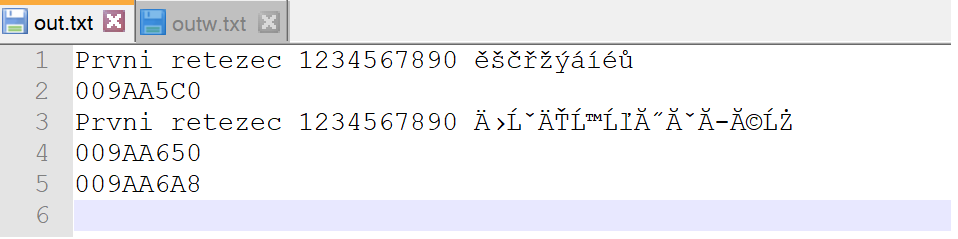
\includegraphics[width=\textwidth]{img/datastreams-outtxt.png}
\end{frame}



\begin{frame}[fragile]
\frametitle{wofstream - různé formáty textu}
\begin{yesblock}
\begin{lstlisting}
wofstream outputFile{ "outw.txt" };
// char
outputFile << "Prvni retezec 1234567890 ěščřžýáíéů" << endl;
// wchar_t
outputFile << L"Prvni retezec 1234567890 ěščřžýáíéů" << endl;
// utf-8 (char)
outputFile << u8"Prvni retezec 1234567890 ěščřžýáíéů" << endl;
// utf-16 (char16_t)
outputFile << u"Prvni retezec 1234567890 ěščřžýáíéů" << endl;
// utf-32 (char32_t)
outputFile << U"Prvni retezec 1234567890 ěščřžýáíéů" << endl;
outputFile.close();
\end{lstlisting}
\end{yesblock}
\end{frame}


\begin{frame}[fragile]
\begin{block}{}
Náhled v režimu ANSI (cp1250)
\begin{itemize}
\item korektně není zapsán žádný řetězec!
\item i u \lstinline|wchar_t| došlo k ořezu diakritických znaků
\end{itemize}
\end{block}
\vskip 1ex
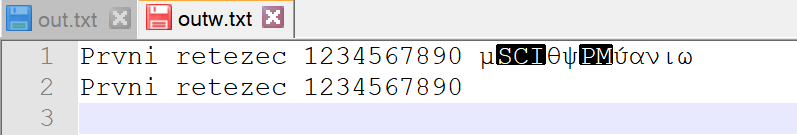
\includegraphics[width=\textwidth]{img/datastreams-outwtxt.png}
\end{frame}



\begin{frame}[fragile]
\frametitle{basic\_ofstream<char16\_t> - různé formáty textu}
\begin{yesblock}
\begin{lstlisting}
// utf-16 (char16_t)
std::basic_ofstream<char16_t> outputFile{ "out16.txt" };
outputFile << u"Prvni retezec 1234567890 ěščřžýáíéů" << endl;
outputFile.close();
\end{lstlisting}
\end{yesblock}
\end{frame}


\begin{frame}[fragile]
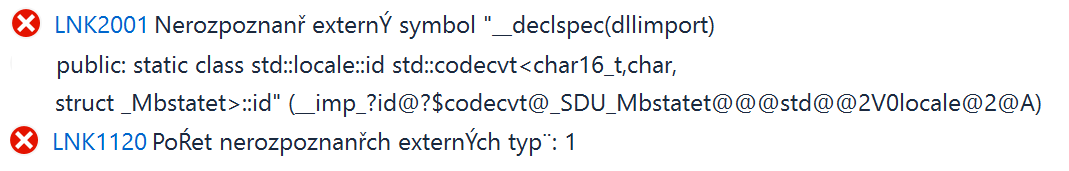
\includegraphics[width=\textwidth]{img/datastreams-char16terror.png}
\end{frame}

\begin{frame}[fragile]
\begin{block}{}
\begin{itemize}
\item V rámci paměti lze používat řetězce v kódování nativním kódování, UTF-8, UTF-16, UTF-32
\item V prostředí VS lze do souboru pouze zapisovat v nativním kódováním nebo v UTF-8
\end{itemize}
\end{block}
\end{frame}





\pkapitola{Binární soubory}




\begin{frame}[fragile]
\frametitle{Zápis binárního souboru -- struktura}
\begin{yesblock}
\begin{lstlisting}
struct JednoduchaStruktura {
	int a;
	int b;
	int c;
};

void testZapisACteniBinarne() {
	JednoduchaStruktura abc{ 1, 2, 3 };
	
	ofstream binFile{ "out.bin" };
	binFile.write((const char*)&abc, sizeof abc);
	binFile.close();
}

\end{lstlisting}
\end{yesblock}
\end{frame}


\begin{frame}[fragile]

\begin{block}{}
Náhled v HEX editoru
\begin{itemize}
\item \lstinline|sizeof(int) == 4| 
\item \lstinline|sizeof(JednoduchaStruktura) == 3*4 == 12|
\item OK
\item Pozor na přenos souboru na jinou platformu -- pořadí bajtů ve skupině je nyní little-endian
\begin{itemize}
\item Na systému big-endian by byly načteny hodnoty 16 777 216, 33 554 432, 50 331 648
\end{itemize}
\end{itemize}
\end{block}
\vskip 1ex
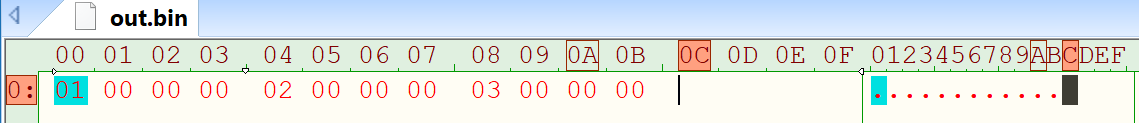
\includegraphics[width=\textwidth]{img/datastreams-bin1.png}
\end{frame}










\begin{frame}[fragile]
\frametitle{Zápis binárního souboru -- struktura}
\begin{yesblock}
\begin{lstlisting}
struct SlozitejsiStruktura {
	JednoduchaStruktura& ref;
	JednoduchaStruktura* ptr;
};

void testZapisACteniBinarne() {
	JednoduchaStruktura abc{ 1, 2, 3 };
	SlozitejsiStruktura structure{ abc, &abc };

	ofstream binFile{ "out.bin" };
	binFile.write((const char*)&structure, sizeof structure);
	binFile.close();
}
\end{lstlisting}
\end{yesblock}
\end{frame}


\begin{frame}[fragile]

\begin{block}{}
Náhled v HEX editoru
\begin{itemize}
\item \lstinline|sizeof(JednoduchaStruktura) == 12|
\item Velikost souboru == 8
\item Není OK
\item Reference i ukazatele jsou v paměti reprezentovány stejně
\begin{itemize}
\item Ukazatel (32/64 bitové číslo) na adresu do paměti
\item Binární zápis pouze zapíše hodnotu (tj. tu adresu), kterou ve struktuře přečte
\end{itemize}
\end{itemize}
\end{block}
\vskip 1ex
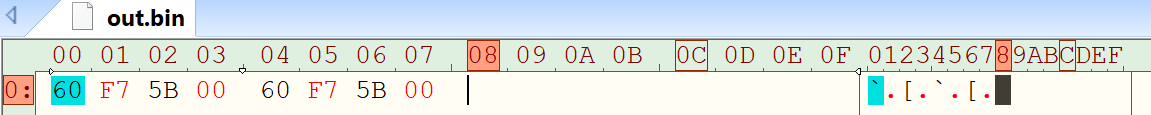
\includegraphics[width=\textwidth]{img/datastreams-bin2.png}
\end{frame}









\begin{frame}[fragile]
\frametitle{Zápis binárního souboru -- struktura}
\begin{yesblock}
\begin{lstlisting}
struct NevyrovnanaStruktura {
	char a;
	int b;
	char c;
	double d;
};

void testZapisACteniBinarne() {
	NevyrovnanaStruktura structure{ 0x99, 0x12345678, 0x99, 3.14};

	ofstream binFile{ "out.bin" };
	binFile.write((const char*)&structure, sizeof structure);
	binFile.close();
}
\end{lstlisting}
\end{yesblock}
\end{frame}


\begin{frame}[fragile]

\begin{block}{}
Náhled v HEX editoru
\begin{itemize}
\item \lstinline|sizeof(char)+sizeof(int)+sizeof(char)+sizeof(double) == 1+4+1+8 == 14|
\item Velikost souboru == 24
\item OK? Proč je větší?
\item Kompilátor automaticky zarovnává struktury (a třídy) v paměti, tak aby procesor přistupoval k adresám, které jsou násobky 4/8 bajtů a bylo dosaženo vyššího výkonu
\begin{itemize}
\item Stejný program bude strukturu znovu schopen načíst.
\item Stejný program zkompilovány jiným kompilátorem může na načítání selhat!
\end{itemize}

\end{itemize}
\end{block}
\vskip 1ex
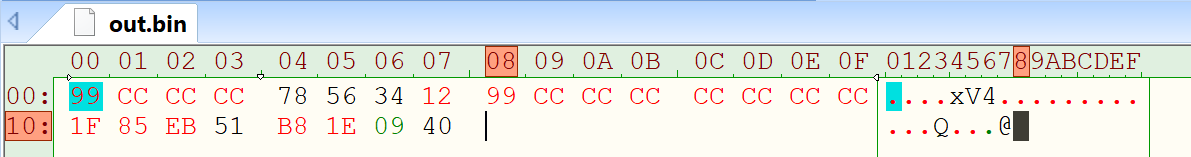
\includegraphics[width=\textwidth]{img/datastreams-bin3.png}
\end{frame}









\begin{frame}[fragile]
\frametitle{Zápis binárního souboru -- struktura}
\begin{yesblock}
\begin{lstlisting}
struct Struktura {
	string retezec;
};

void testZapisACteniBinarne() {
	Struktura structure{ "ahoj svete" };

	ofstream binFile{ "out.bin" };
	binFile.write((const char*)&structure, sizeof structure);
	binFile.close();
}
\end{lstlisting}
\end{yesblock}
\end{frame}


\begin{frame}[fragile]

\begin{block}{}
Náhled v HEX editoru
\begin{itemize}
\item Velikost souboru == 29
\item OK? Proč je to tolik?
\item Je to třída a nese nějaké atributy navíc, ale jinak to jde zapsat i načíst

\end{itemize}
\end{block}
\vskip 1ex
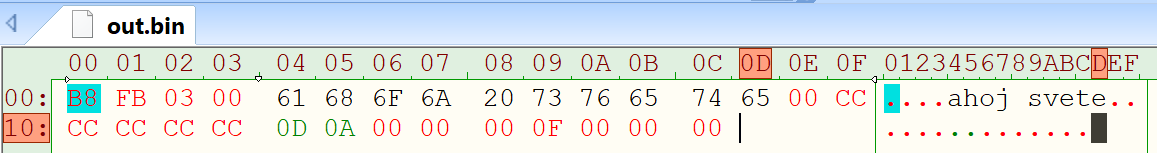
\includegraphics[width=\textwidth]{img/datastreams-bin4.png}
\end{frame}








\begin{frame}[fragile]
\frametitle{Zápis binárního souboru -- struktura}
\begin{yesblock}
\begin{lstlisting}
struct Struktura {
	string retezec;
};

void testZapisACteniBinarne() {
	Struktura structure{ "ahoj svete, dneska je moc pekne!" };

	ofstream binFile{ "out.bin" };
	binFile.write((const char*)&structure, sizeof structure);
	binFile.close();
}
\end{lstlisting}
\end{yesblock}
\end{frame}


\begin{frame}[fragile]

\begin{block}{}
Náhled v HEX editoru
\begin{itemize}
\item Velikost souboru == 28
\item OK? Ne!
\item Text není uložen v souboru!

\end{itemize}
\end{block}
\vskip 1ex
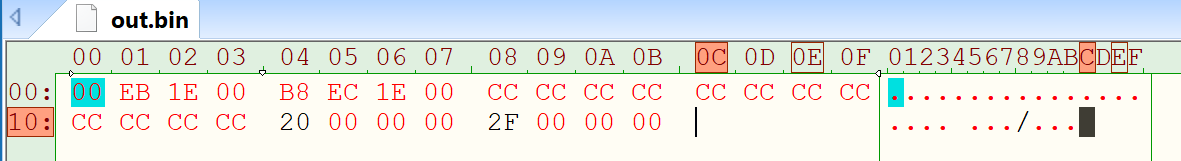
\includegraphics[width=\textwidth]{img/datastreams-bin5.png}
\end{frame}

\begin{frame}[fragile]
\begin{block}{Implementace std::string v knihovně}
\begin{itemize}
\item Liší se dle autora knihovny
\item Někde je využívána přímo dynamicky alokovaná paměť
\item Někde je používán hybridní přístup
\begin{itemize}
\item Pro krátké řetězce (do 16 znaků) je přímo ve třídě staticky alokované pole, kam se uloží znaky
\item Delší řetězce vyžadují alokaci samostatného paměťového bloku a do struktury je uložen ukazatel
\item[] 
\item Tento přístup umožňuje předcházet dvojí alokaci paměti pro krátké řetězce
\item Je využíván i v rámci knihovny od Microsoftu
\end{itemize}
\end{itemize}
\end{block}
\end{frame}


\begin{frame}[fragile]

\begin{block}{Zápis struktur do souboru}
Lze při splnění podmínek:
\begin{itemize}
\item struktura neobsahuje referenční nebo ukazatelové atributy
\item program má ošetřenou přenositelnost (little-endian/big-endian) pro případ přesunu na jinou platformu
\item program má ošetřené zarovnání struktur pro případ přesunu na jiný kompilátor/platformu
\end{itemize}
\vskip 1ex
Nelze tedy přímo zapisovat struktury u kterých si nejsme jisti splněním těchto podmínek (\lstinline|std::vector, std::string|, \ldots)

\end{block}
\end{frame}



\zkouskove
